\documentclass[11pt]{article}
\usepackage{minted}
\usepackage{graphicx}

\usepackage{classTools}

\begin{document}

\psHeader{4}{Wed Oct. 18, 2023 (11:59pm)}


\textbf{Your name:} Cory Zimmerman

\textbf{Collaborators:} None

\textbf{No. of late days used on previous psets:} 0

\textbf{No. of late days used after including this pset:} 0

\begin{enumerate}
    \item (Randomized Algorithms in Practice)  
    \begin{enumerate}
        \item Implement Randomized QuickSelect, filling in the template we have given you in the \href{https://github.com/Harvard-CS-120/cs120/tree/main/fall2023/psets}{Github repository}.  
        \begin{quote}
            \color{purple}
            Done.
        \end{quote}

        \item 
        In the repository, we have given you datasets $x_n$ of
        key-value pairs of varying sizes to experiment with: data set $x_n$ is of size $n$.  For each dataset $x_n$ and any given number $k$, you will compare two ways of answering the $k$ selection queries
        \textsc{Select}$(x_n,[n/k])$, \textsc{Select}$(x_n,[2n/k]), \ldots$, \textsc{Select}$(x_n,[(k-1)n/k])$ on $x_n$, where $[\cdot]$ denotes rounding to the nearest integer:
        \begin{enumerate}
            \item Running Randomized QuickSelect $k$ times
            \item Running MergeSort (provided in the repository) once and using the sorted array to answer the $k$ queries
        \end{enumerate}
        Specifically, you will compare the {\em distribution} of runtimes of the two approaches for a given pair $(n,k)$ by running each approach many times and creating density plots of the runtimes.  The runtimes will vary because Randomized QuickSelect  is randomized, and because of variance in the execution environment (e.g. what other processes are running on your computer during each execution). \vspace{1.5mm}
        
        We have provided you with the code for plotting. Before plotting, you will need to implement MergeSortSelect, which extends MergeSort to answer $k$ queries. Your goal is to use these experiments and the resulting density plots to propose a value for $k$, denoted $k^*_n$, at which you should switch over from Randomized QuickSelect to MergeSort for each given value of $n$. Do this by experimenting with the parameters for $k$ (code is included to generate the appropriate queries once the $k$s are provided) and generate a plot for each experiment.  Explain the rationale behind your choices, and submit a few density plots for each value of $n$ to support your reasoning.  (There is not one right answer, and it may depend on your particular implementation of QuickSelect.) 

        \begin{quote}
        \color{purple}
        \vspace{1em}
           QuickSelect v. MergeSortSelect on $k = [24, 32, 40, 48, 56]$. \newline
           \newline
            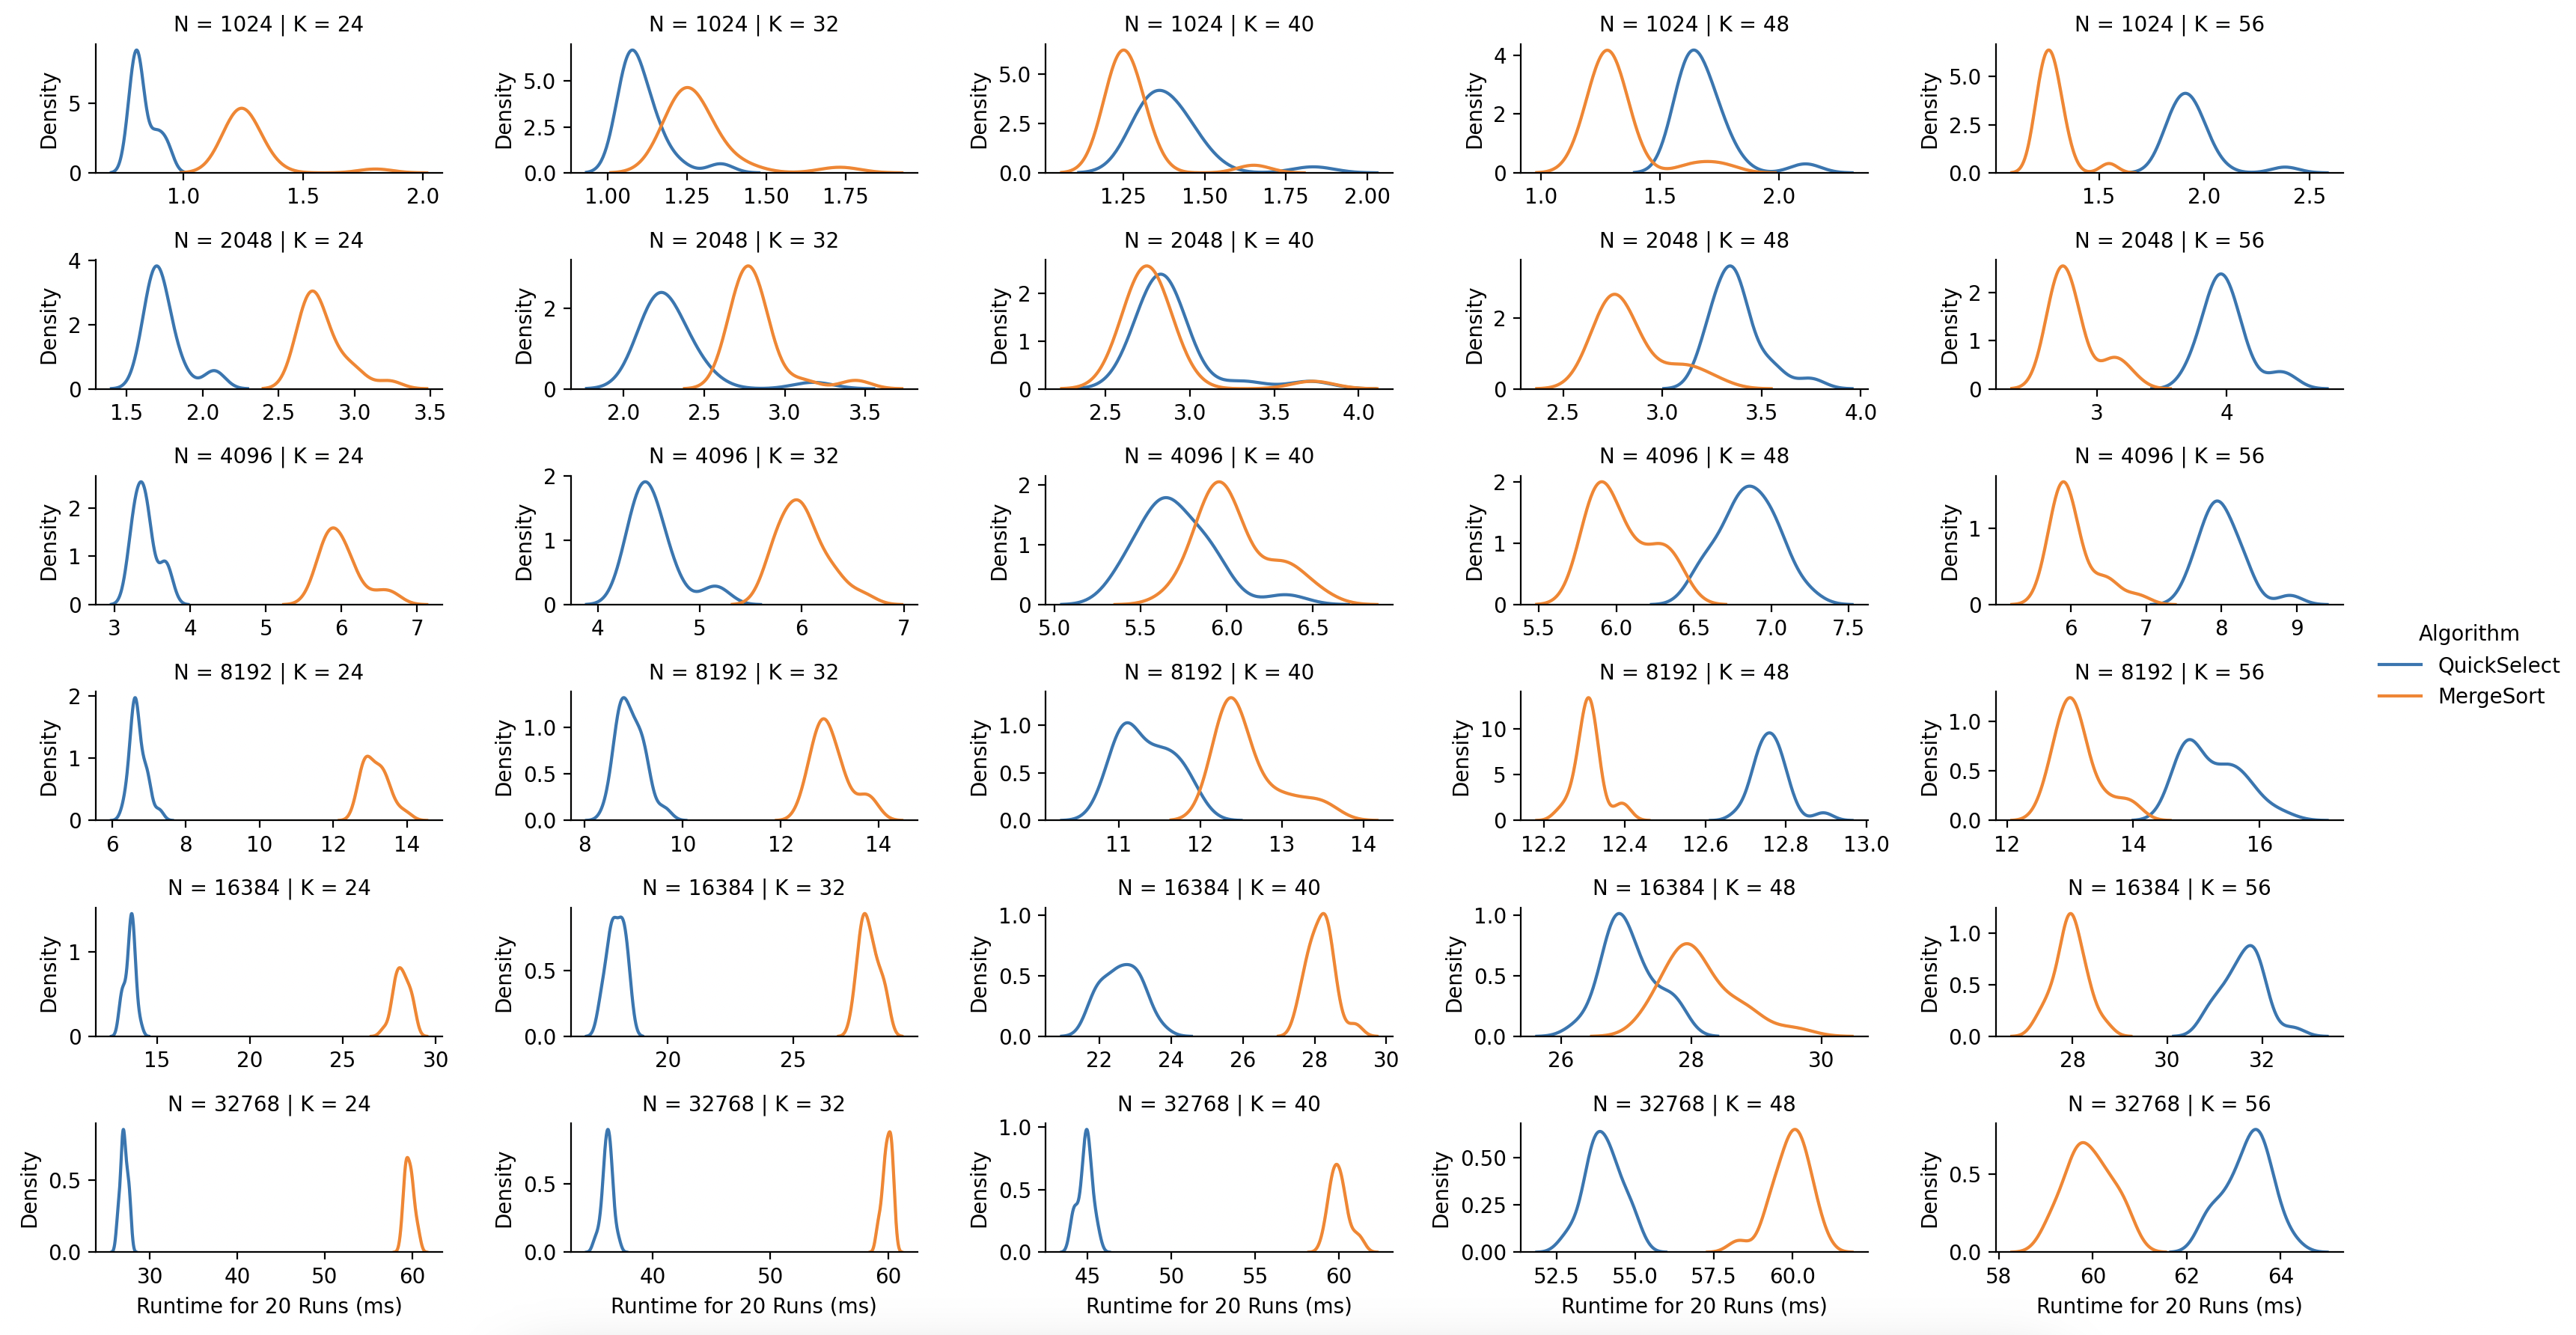
\includegraphics[scale=0.2]{qs [24, 32, 40, 48, 56].png} 
           \newline
           QuickSelect v. MergeSortSelect on $k = [32, 38, 44, 50, 56]$. \newline
           \newline
            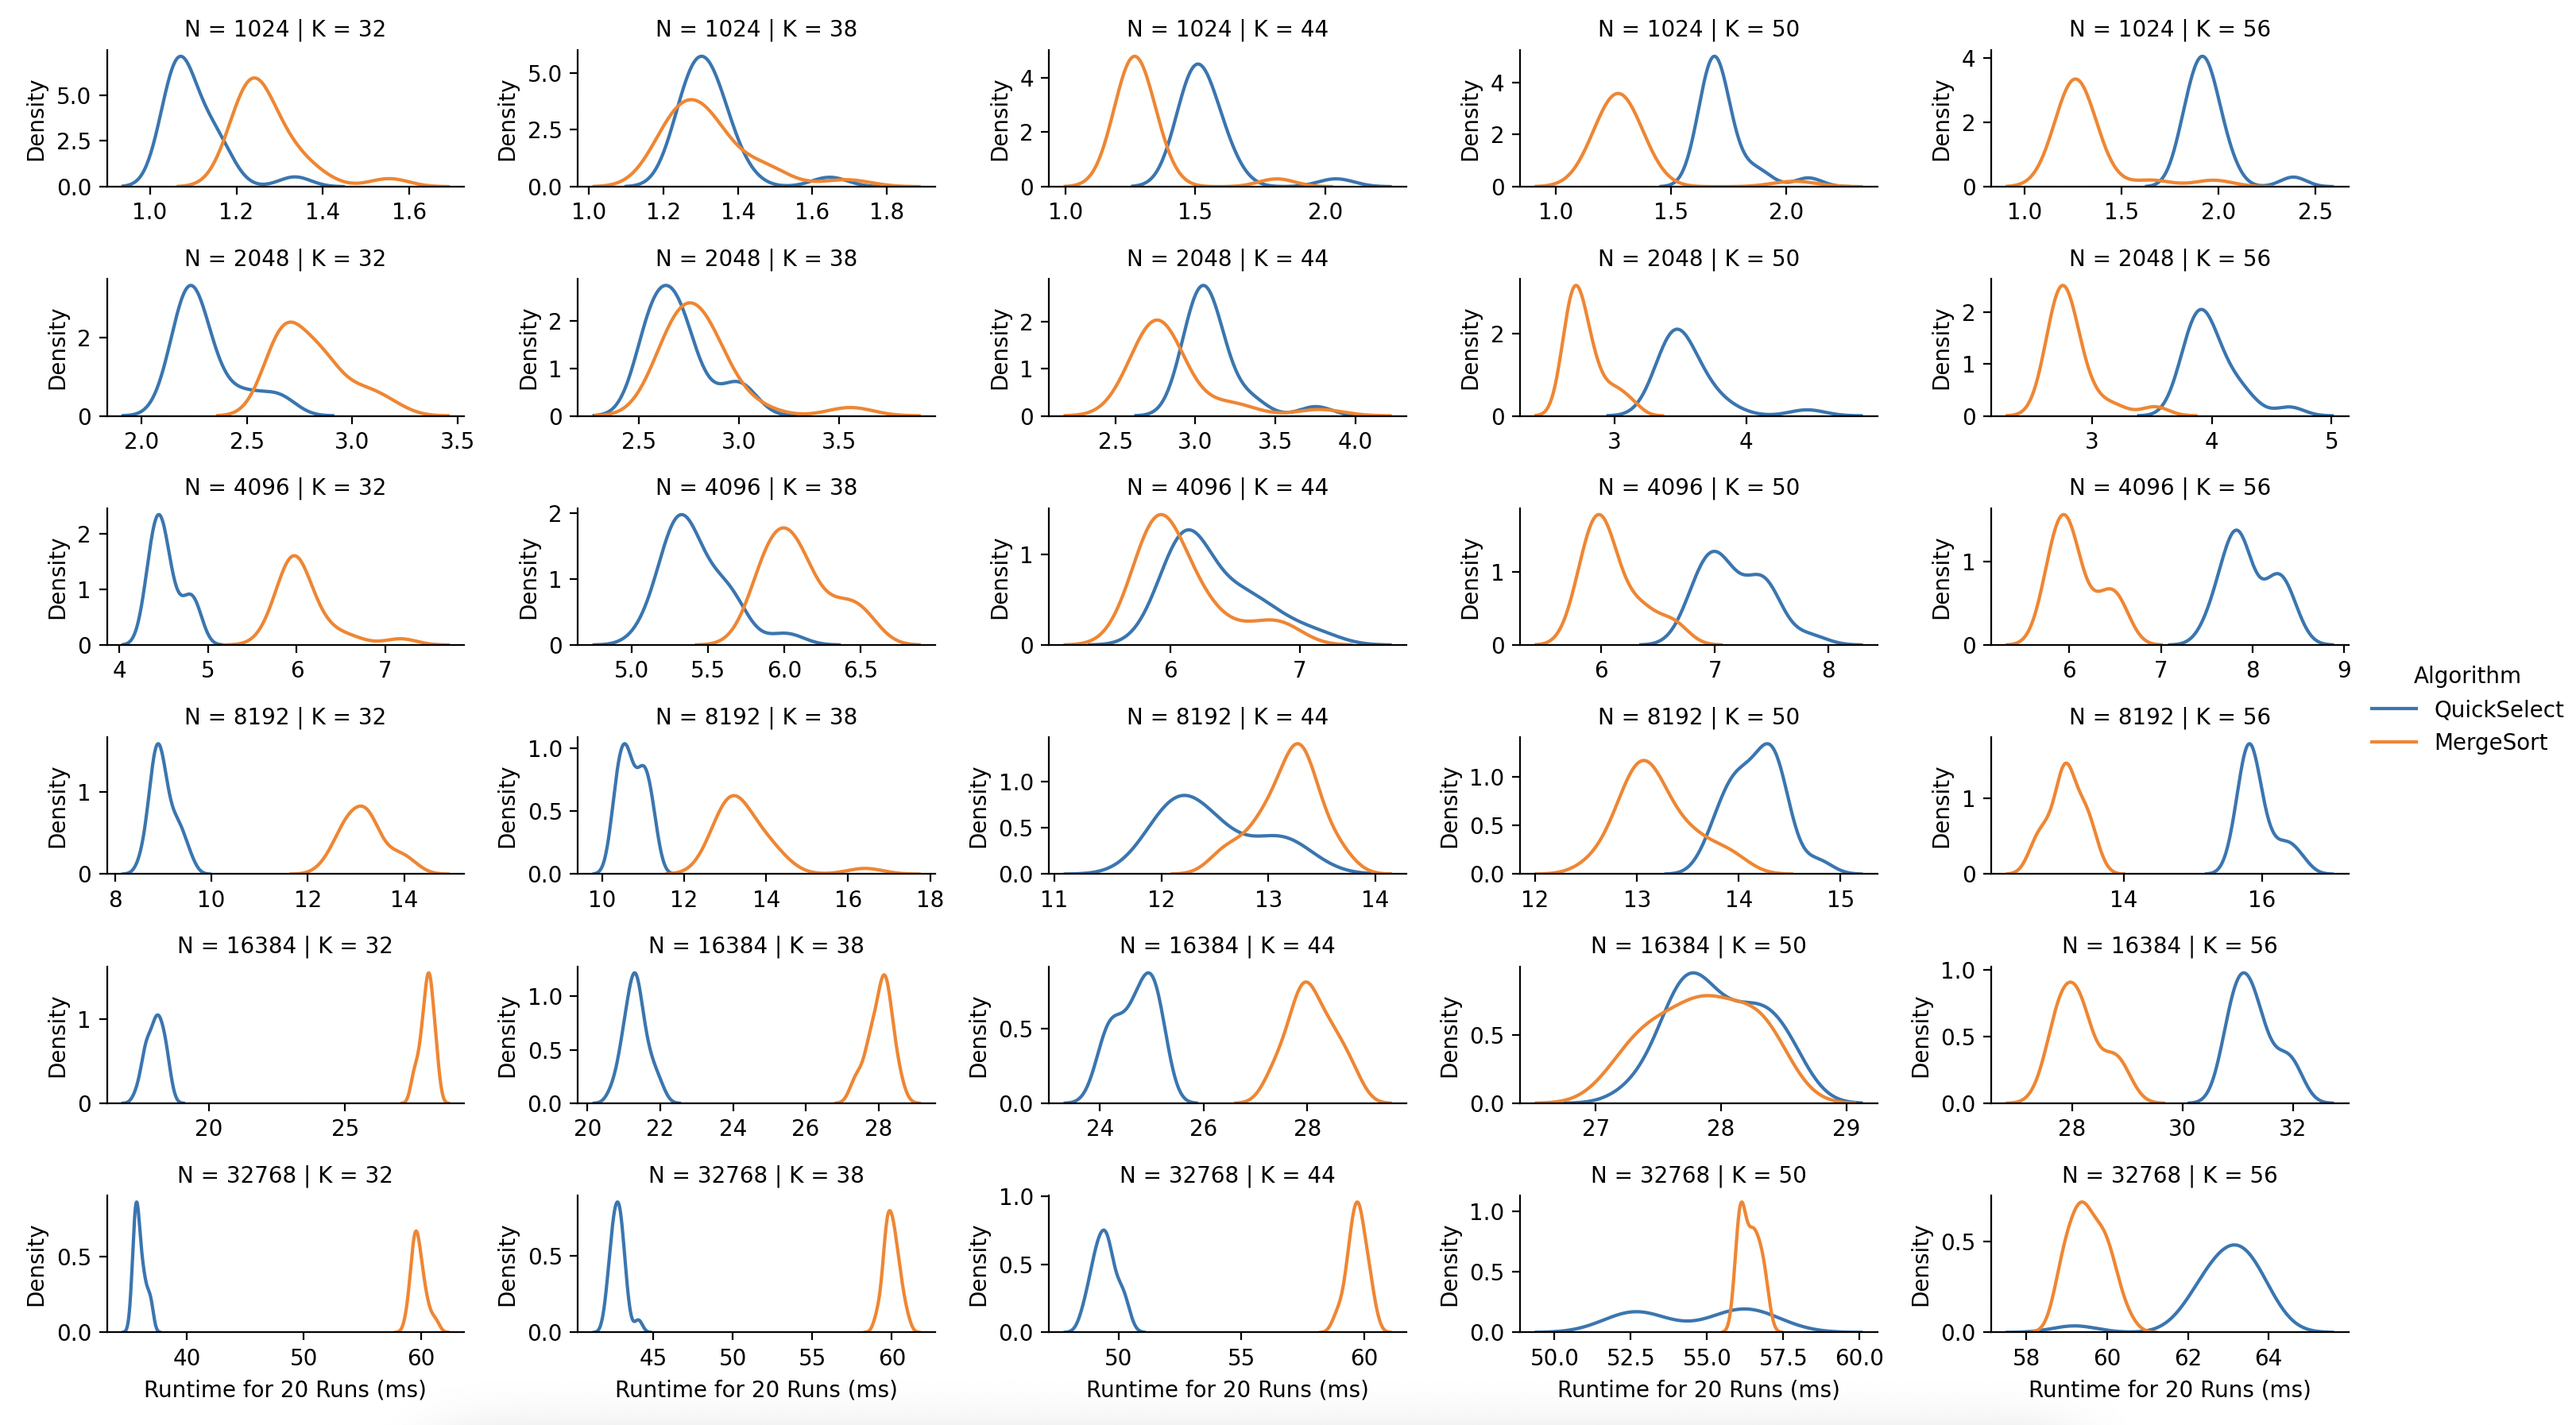
\includegraphics[scale=0.2]{qs [32, 38, 44, 50, 56].png} 
           \newline
           Based on the graphs, I'll make the following estimations for $k$ and $n$:
           \begin{itemize}
               \item $n = 1024$: QuickSelect is faster until about $k = 38$, after which MergeSortSelect is faster.
               \item $n = 2048$: QuickSelect is faster until about $k = 40$.
               \item $n = 4096$: QuickSelect is faster until about $k = 42$.
               \item $n = 8192$: QuickSelect is faster until about $k = 46$.
               \item $n = 16384$: QuickSelect is faster until about $k = 48$.
               \item $n = 32768$: QuickSelect is faster until about $k = 50$, after which MergeSortSelect is faster. There was a lot of noise in this estimation, though.
           \end{itemize}
           \vspace{1em}
           Overall, it's consistent with expectations that QuickSelect is faster for a lower $k$ value, and MergeSortSelect is faster when we're running more queries. As $n$ increases, the difference between the expected $O(n)$ runtime for QuickSelect and the $O(n \log n)$ runtime for MergeSort becomes more pronounced, which pushes up the value of $k$.
           
        \end{quote}

        \item Extrapolate to come up with a simple functional form for $k^*_n$, e.g. something like $k^*(n)=3\sqrt{n}+6$ or $k^*(n)=10\log n$. (Again there is not one right answer.)

        \begin{quote}
            \color{purple}
            Based on the results above, I'd suggest an approximation function around $k^*(n) = 2 \log_2 (n) + 18$. I'd probably need to check if this holds up at much higher values of $n$, but it seems approprate in this range of $n$.
        \end{quote}

        \item (*optional)  One way to improve Randomized QuickSelect is to choose a pivot more carefully than by picking a uniformly random element from the array. A possible approach is to use the \textit{\textbf{median-of-3}} method: choose the pivot as the median of a set of 3 elements randomly selected from the array. Add Median-of-3 QuickSelect to the experimental comparisons you performed above and interpret the results.
        \begin{quote}
            \color{purple}
           QuickSelect v. MergeSortSelect on $k = [24, 32, 40, 48, 56]$ with Median of Three pivot selection. \newline
           \newline
            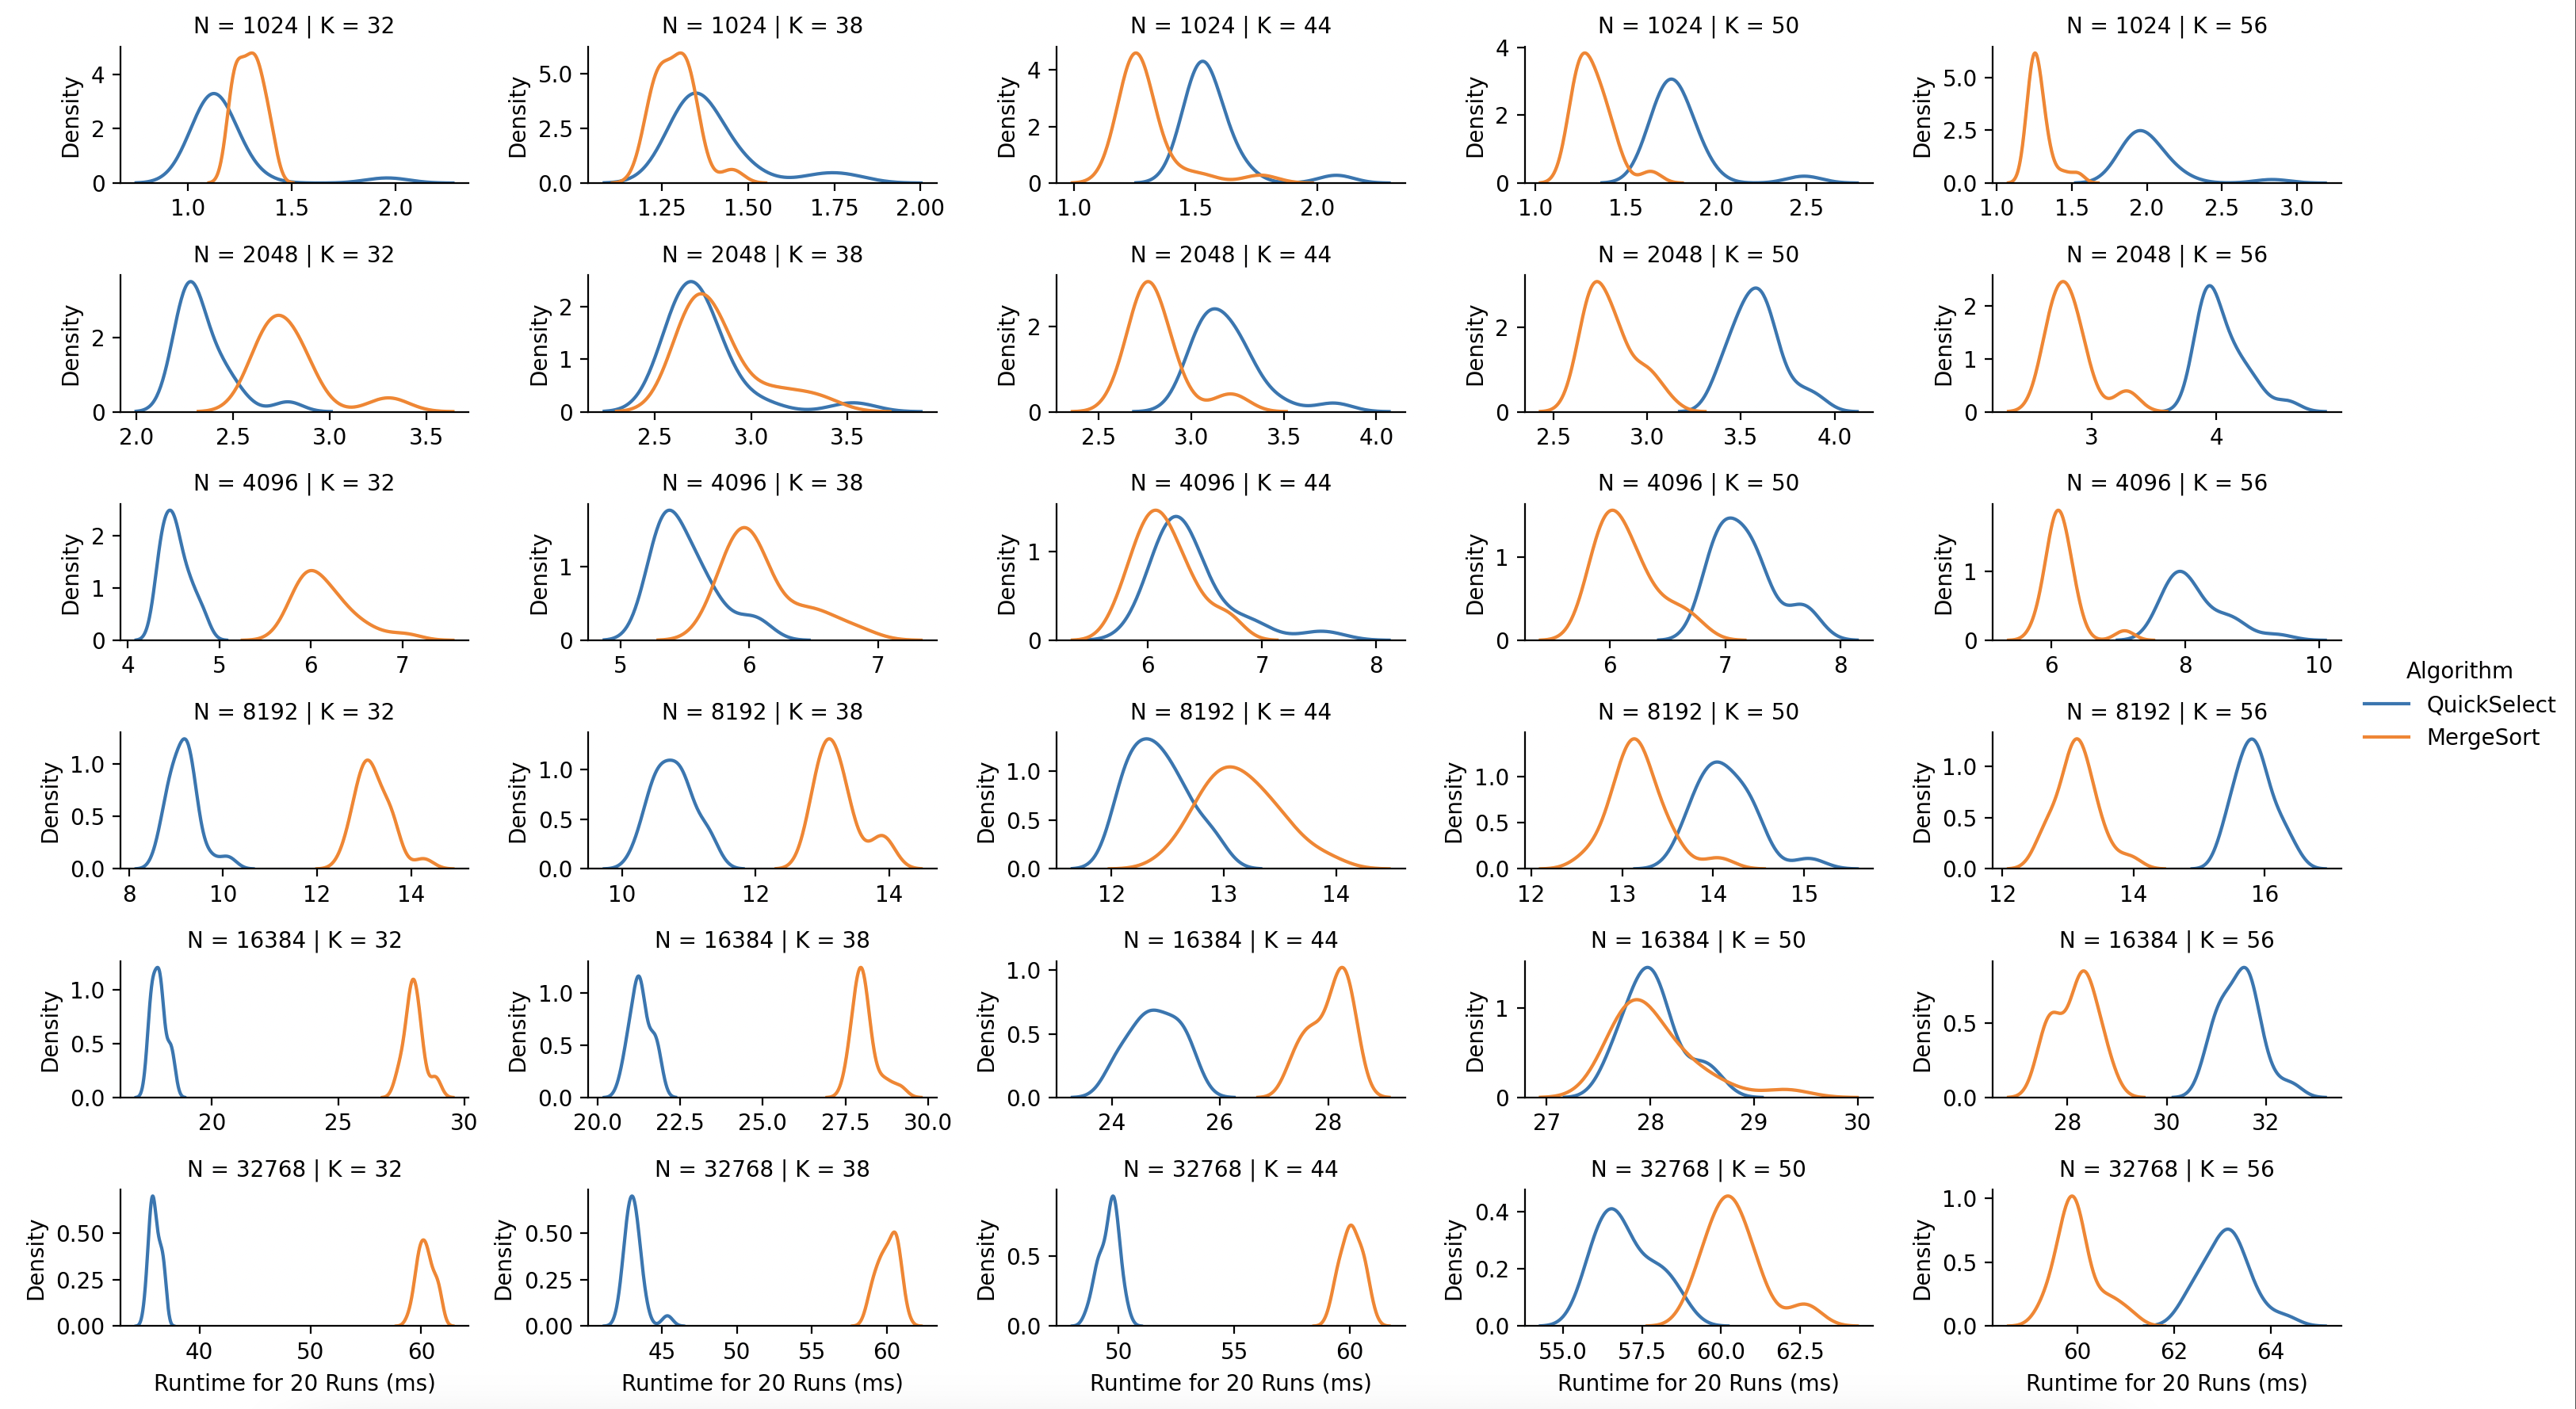
\includegraphics[scale=0.2]{qs med [32, 38, 44, 50, 56].png} 
           \newline
           It seems that Median of Three is a bit faster than with the purely random pivot, but the total performance improvement isn't exceedingly pronounced. However, the peaks for QuickSelect are now much sharper, especially with high $n$ and high $k$. So, while the measured $k$ values from earlier don't seem to change much, confidence in their correctness can be much greater with these changes. Overall, Median of Three seems to have made QuickSelect much more reliable as an $O(n)$ expected time algorithm.
        \end{quote}

    \end{enumerate}


    \item (Dictionaries and Hash Tables) 
    Recall the DuplicateSearch problem from Lecture 3. Show that DuplicateSearch can be solved by a Las Vegas algorithm with expected runtime $O(n)$ using a dictionary data structure.  (You can quote the runtimes of the implementation of a dictionary data structure from Lecture 9 without proof.) (No formal probabilistic analysis of the runtime is necessary.)
    \begin{quote}
        \color{purple}
        To solve DuplicateSearch, first recall the definition of the problem. It must accept a list of real numbers and return a duplicate number from the list if one exists. Otherwise, $\bot$ is returned. \newline 

        Consider the following algorithm to solve this problem:
        \begin{enumerate}
            \item Initialize an empty hash table data structure.
            \item For every input number:
            \begin{itemize}
                \item Search for this number as a key in the hash table. If the key is found, return this number.
                \item Else, insert the number as a key into the hash table. The value mapped to the key can be arbitrary.
            \end{itemize}
            \item Return $\bot$.
        \end{enumerate}

        \vspace{1em}
        \textbf{Correctness}: \newline
        Let an array $input$ represent any valid input. This algorithm considers every number in $input$. If the number has not been seen before, it is not in the Hash Table. We add it to the table and move on. If it has been seen before, it is in the Hash Table, in which case the duplicate element has been found and is returned. If no duplicate element is ever found, the algorithm returns $\bot$. In this way, the algorithm returns a valid output for every valid input, so it must be correct.
        
        \vspace{1em}
        \textbf{Runtime}: \newline
        This is a Las Vegas algorithm because it depends on a Hash Table, a Las Vegas data structure. Because the algorithm iterates over every input element, if the input has length $n$, the algorithm runs in at least $O(n)$ time. From the proofs in class, assert that the runtime of the $insert$ and $query$ methods of the Hash Table data structure are expected to take an average of $O(1)$ time assuming the load of the table is properly managed. Running an expected constant time operation $n$ times yields an expected $O(n)$ runtime for this algorithm. The time for a given $insert$ or $query$ operation may degenerate, causing an outlier runtime. However, because the $insert$ and $query$ methods are themselves Las Vegas algorithms, they'll never fail. Because of that, the runtime of this algorithm may degenerate, but it will never fail.

        
    \end{quote}

    \item  (Rotating Walks)  
    Suppose we are given $k$ digraphs on the same vertex set, $G_0=(V,E_0), G_1=(V,E_1), \ldots, G_{k-1}=(V,E_{k-1})$.  For vertices $s,t\in V$, a {\em rotating walk} with respect to $G_0,\ldots,G_{k-1}$ from $s$ to $t$ is a sequence of vertices $v_0,v_1,\ldots,v_{\ell}$ such that $v_0=s$, $v_\ell=t$, and $(v_i,v_{i+1})\in E_{i \bmod k}$ for $i=0,\ldots,\ell-1$.  That is, we are looking for walks that rotate between the digraphs $G_0,G_1,\ldots,G_{k-1}$ in the edges used.
    \begin{enumerate}
        \item Show that the problem of finding a Shortest Rotating Walk from $s$ to $t$ with respect to $G_0,\ldots,G_{k-1}$ 
        can be reduced to Single-Source Shortest Walks via a reduction that makes one oracle call on 
        a digraph $G'$ with $kn$ vertices and $m_0+m_1+\cdots+m_{k-1}$ edges, where $n=|V|$ and $m_i=|E_i|$.
        We encourage you to index the vertices of $G'$ by pairs $(v,j)$ where $v\in V$ and $j\in [k]$. 
        Analyze the running time of your reduction and deduce that the Shortest Rotating Walk can be found in time $O(kn+m_0+\cdots+m_{k-1})$.
        \label{part:ReduceToOrdinary}  To test your reduction and algorithm, try running through the example in Part~\ref{part:BFS}.
        \begin{quote}
            \color{purple}
            \textbf{Algorithm}: \newline 
            The most concrete way to show the solution to a problem is by writing the algorithm in code. I've included that on the next page, so my synthesis here is more limited. In summary, given every input graph, construct a new modified graph, $G'$. The modified graph contains the total number of nodes in all input graphs combined, and nodes in the modified graph are identified by a pair of their original ID and the ID of the graph they came from. For each graph $g$ of graphs $0 \leq g < k - 1$, add edges to $G'$ such that any edge that begins at $a$ and ends at $b$ instead begins at $a$ from graph $g$ and ends at $b$ from graph $g + 1$ mod $k$. In this way, the edges point only to the nodes in the next rotation, and any traversal of $G'$ is a valid rotating walk. Once $G$ is constructed, run single source shortest walk from the $(s, 0)$ node pair to find which rotating walk beginning in Graph 0 is the shortest. Return that shortest walk. Because the algorithm considers every possible rotating walk from among all input graphs, as long as the oracle is correct, this algorithm should return a valid output for every valid input, making it correct. (runtime after code)
            \newpage 
\begin{minted}{python}
from typing import Tuple, List, Set

NodeID = int
InputEdge = Tuple[NodeID, NodeID]
InputGraph = Tuple[Set[NodeID], List[InputEdge]]

OriginGraphID = int
ModifiedNodeID = Tuple[NodeID, OriginGraphID]
ModifiedEdge = Tuple[ModifiedNodeID, ModifiedNodeID]
ModifiedGraph = Tuple[Set[ModifiedNodeID], List[ModifiedEdge]]


def single_source_shortest_walk(
    graph: ModifiedGraph,
    start: ModifiedNodeID,
    end: NodeID,
) -> List[ModifiedEdge]:
    # ORACLE CALL
    """This assumes an oracle conceptually similar to single source
    shortest path from class except only the shortest path is returned,
    not the length of every path from v to s.
    It also assumes the oracle can properly operate on (NodeID, GraphID)
    keys to return any such key where NodeID reaches `end`, regardless of
    the ending GraphID. That simplifies the (already long) code."""
    pass


def shortest_rotating_walk(
    input_graphs: List[InputGraph], s: NodeID, t: NodeID
) -> List[ModifiedEdge]:
    modified_graph_nodes: Set[ModifiedNodeID] = set()
    modified_graph_edges: List[ModifiedEdge] = []

    # PREPROCESSING: Create the modified graph
    for graph_num, (graph_nodes, graph_edges) in enumerate(input_graphs):
        # curr_graph_num counts from 0 to k - 1 for k - 1 input graphs
        next_graph_num: int = (graph_num + 1) % (len(input_graphs) - 1)

        for node in graph_nodes:
            # add every node to the modified graph
            modified_node_id: ModifiedNodeID = (node, graph_num)
            modified_graph_nodes.add(modified_node_id)

        for origin, destination in graph_edges:
            # add every edge to the modified graph
            origin_node: ModifiedNodeID = (origin, graph_num)
            destination_node: ModifiedNodeID = (destination, next_graph_num)
            modified_edge: ModifiedEdge = (origin_node, destination_node)
            # notice the origin and destination now pass from one input GraphID
            # to the next
            modified_graph_edges.append(modified_edge)

    modified_graph: ModifiedGraph = (modified_graph_nodes, modified_graph_edges)
    start_node_id: ModifiedNodeID = (s, 0)
    end_node_id: NodeID = t

    # ORACLE CALL
    path = single_source_shortest_walk(modified_graph, start_node_id, end_node_id)

    return path
\end{minted}

            \vspace{2em}
            \textbf{Runtime}: \newline
            In the preprocessing stage, this algorithm visits every vertex in every input graph. 
            Every graph has the same number of vertices, $n$, and there are $k$ graphs, so this step takes $O(kn)$ time. 
            This algorithm also iterates every edge of every graph. If the edges of graphs $0$ through $k - 1$ are represented by $m_0, m_1, \dots, m_{k - 1}$, then that many steps are added to the algorithm, yielding time complexity of $O(kn + m_0 + m_1 + \dots + m_{k - 1})$. 
            In this reduction, we assume the oracle call is constant. Thus, the algorithm reduces to Single Source Shortest Walk with time complexity $O(kn + m_0 + m_1 + \dots + m_{k - 1})$.      
        \end{quote}
        \vspace{1em}
        
        
        \item \label{part:BFS} 
        Run your algorithm from Part~\ref{part:ReduceToOrdinary} (by hand; no programming necessary) on the following pair of graphs $G_0$ and $G_1$ to find the Shortest Rotating Walk from $s=a$ to $t=c$; this will involve solving Single-Source Shortest Walks on a digraph $G'$ with $2\cdot 7=14$ vertices. Fill out the table provided below with the BFS frontier in $G'$ at each iteration, labelling the vertices of $G'$ as $(a, 0),(b, 0),\ldots,(g,0),(a,1),(b,1),\ldots,(g,1)$, and for each vertex $v$ in the table, drawing an arrow in the graph from $v$'s BFS predecessor to $v$. 

            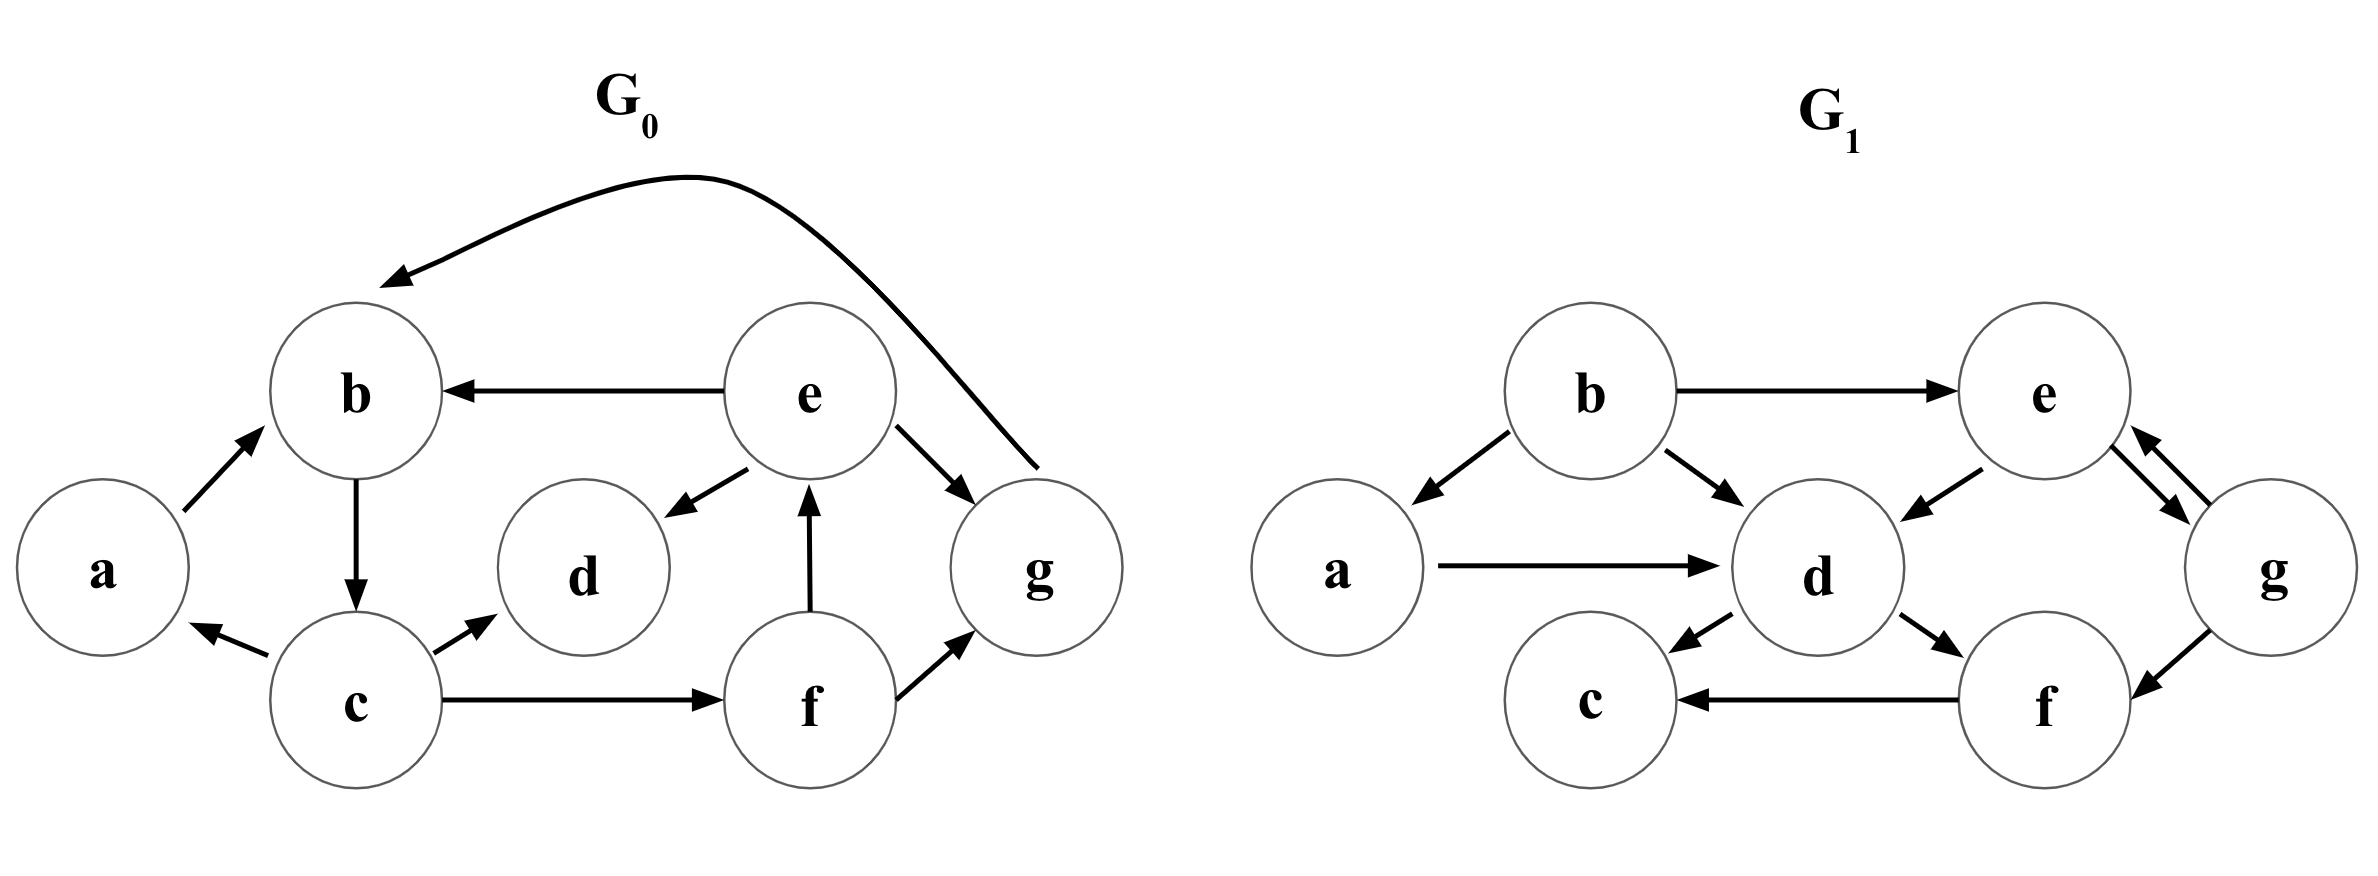
\includegraphics[width=14cm]{ps4_graphs_new.png}
        \begin{table}[ht]
        \centering
        \begin{tabular}{c|c|c}
            $d$ & Frontier $F_d$& Predecessor Relationships \\
            \hline
               0 & (a, 0) &  \{\} \\
               1 & (b, 1) & {(a, 0)} \\
               2 & (d, 0), (e, 0) & {(a, 0), (b, 1)} \\
               3 & (d, 1), (g, 1) & {(a, 0), (b, 1), (e, 0)} \\
               4 & (c, 0), (f, 0) & {(a, 0), (b, 1), (e, 0), (d, 1)} \\
        \end{tabular}
        \end{table}
       \newline
        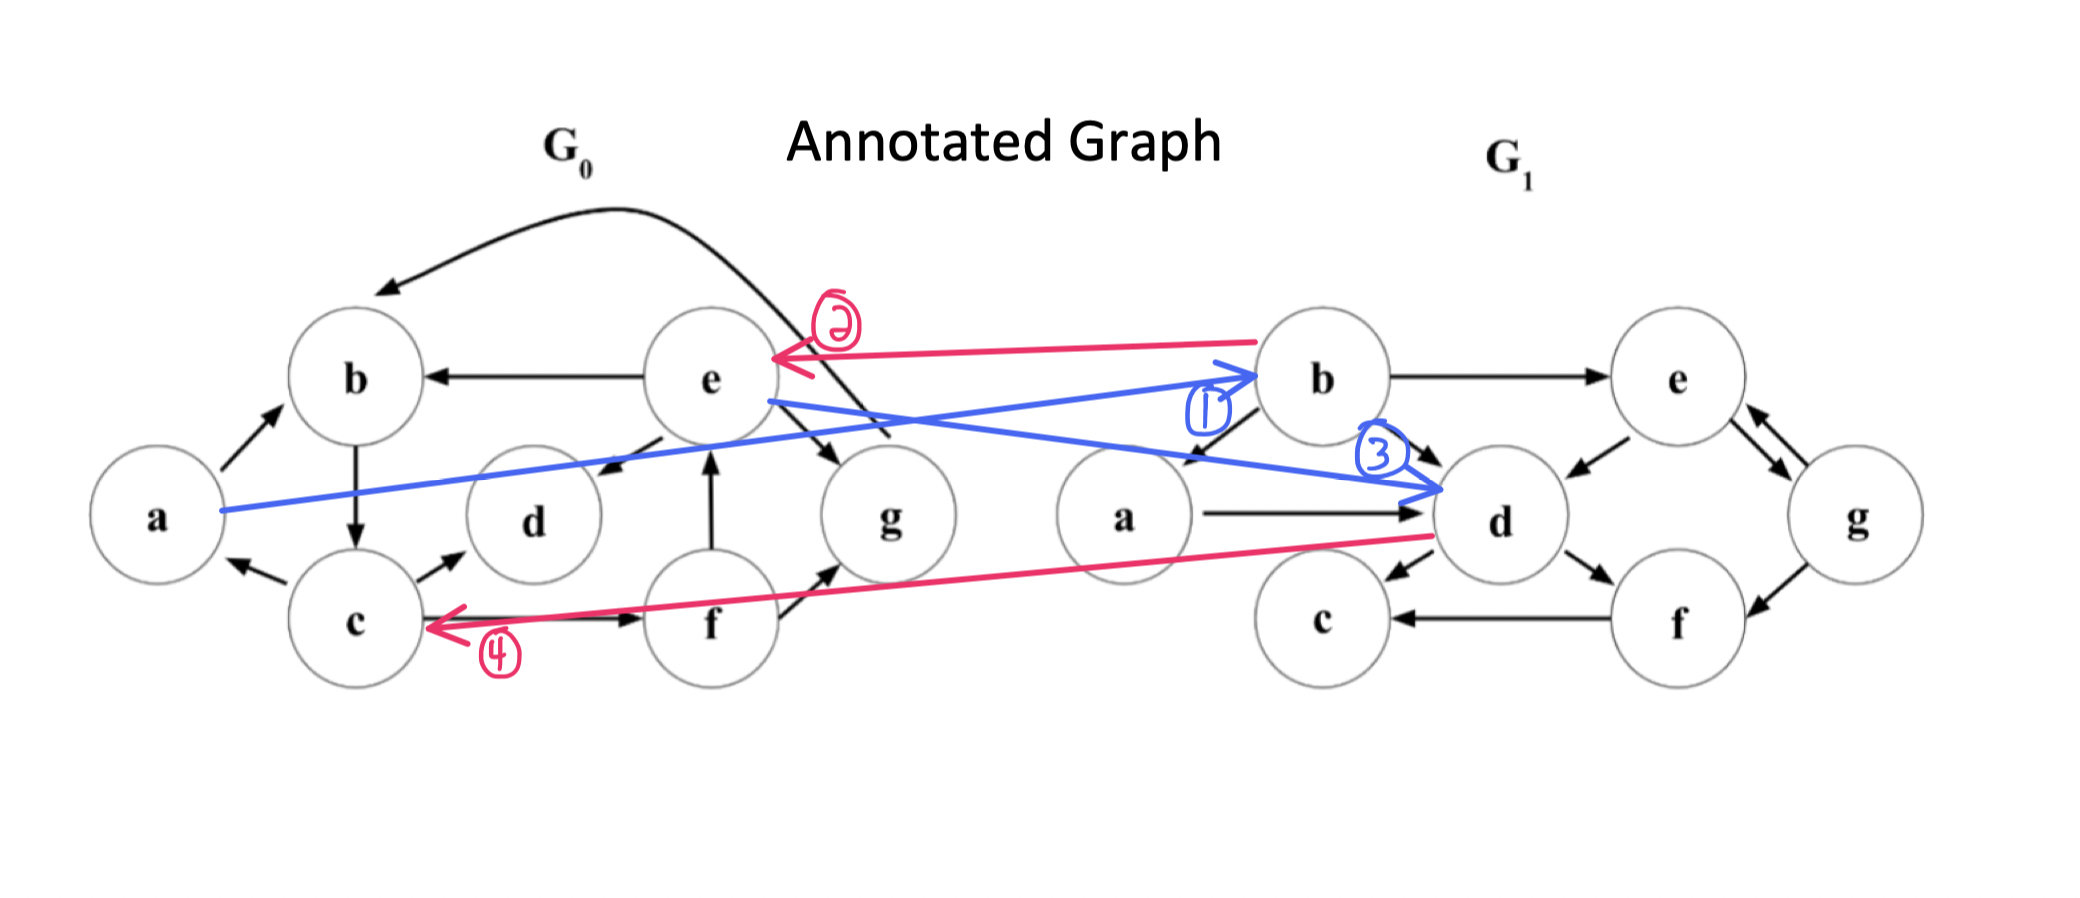
\includegraphics[scale=0.4]{3 b 1.png} 
       \newline
       \newline
        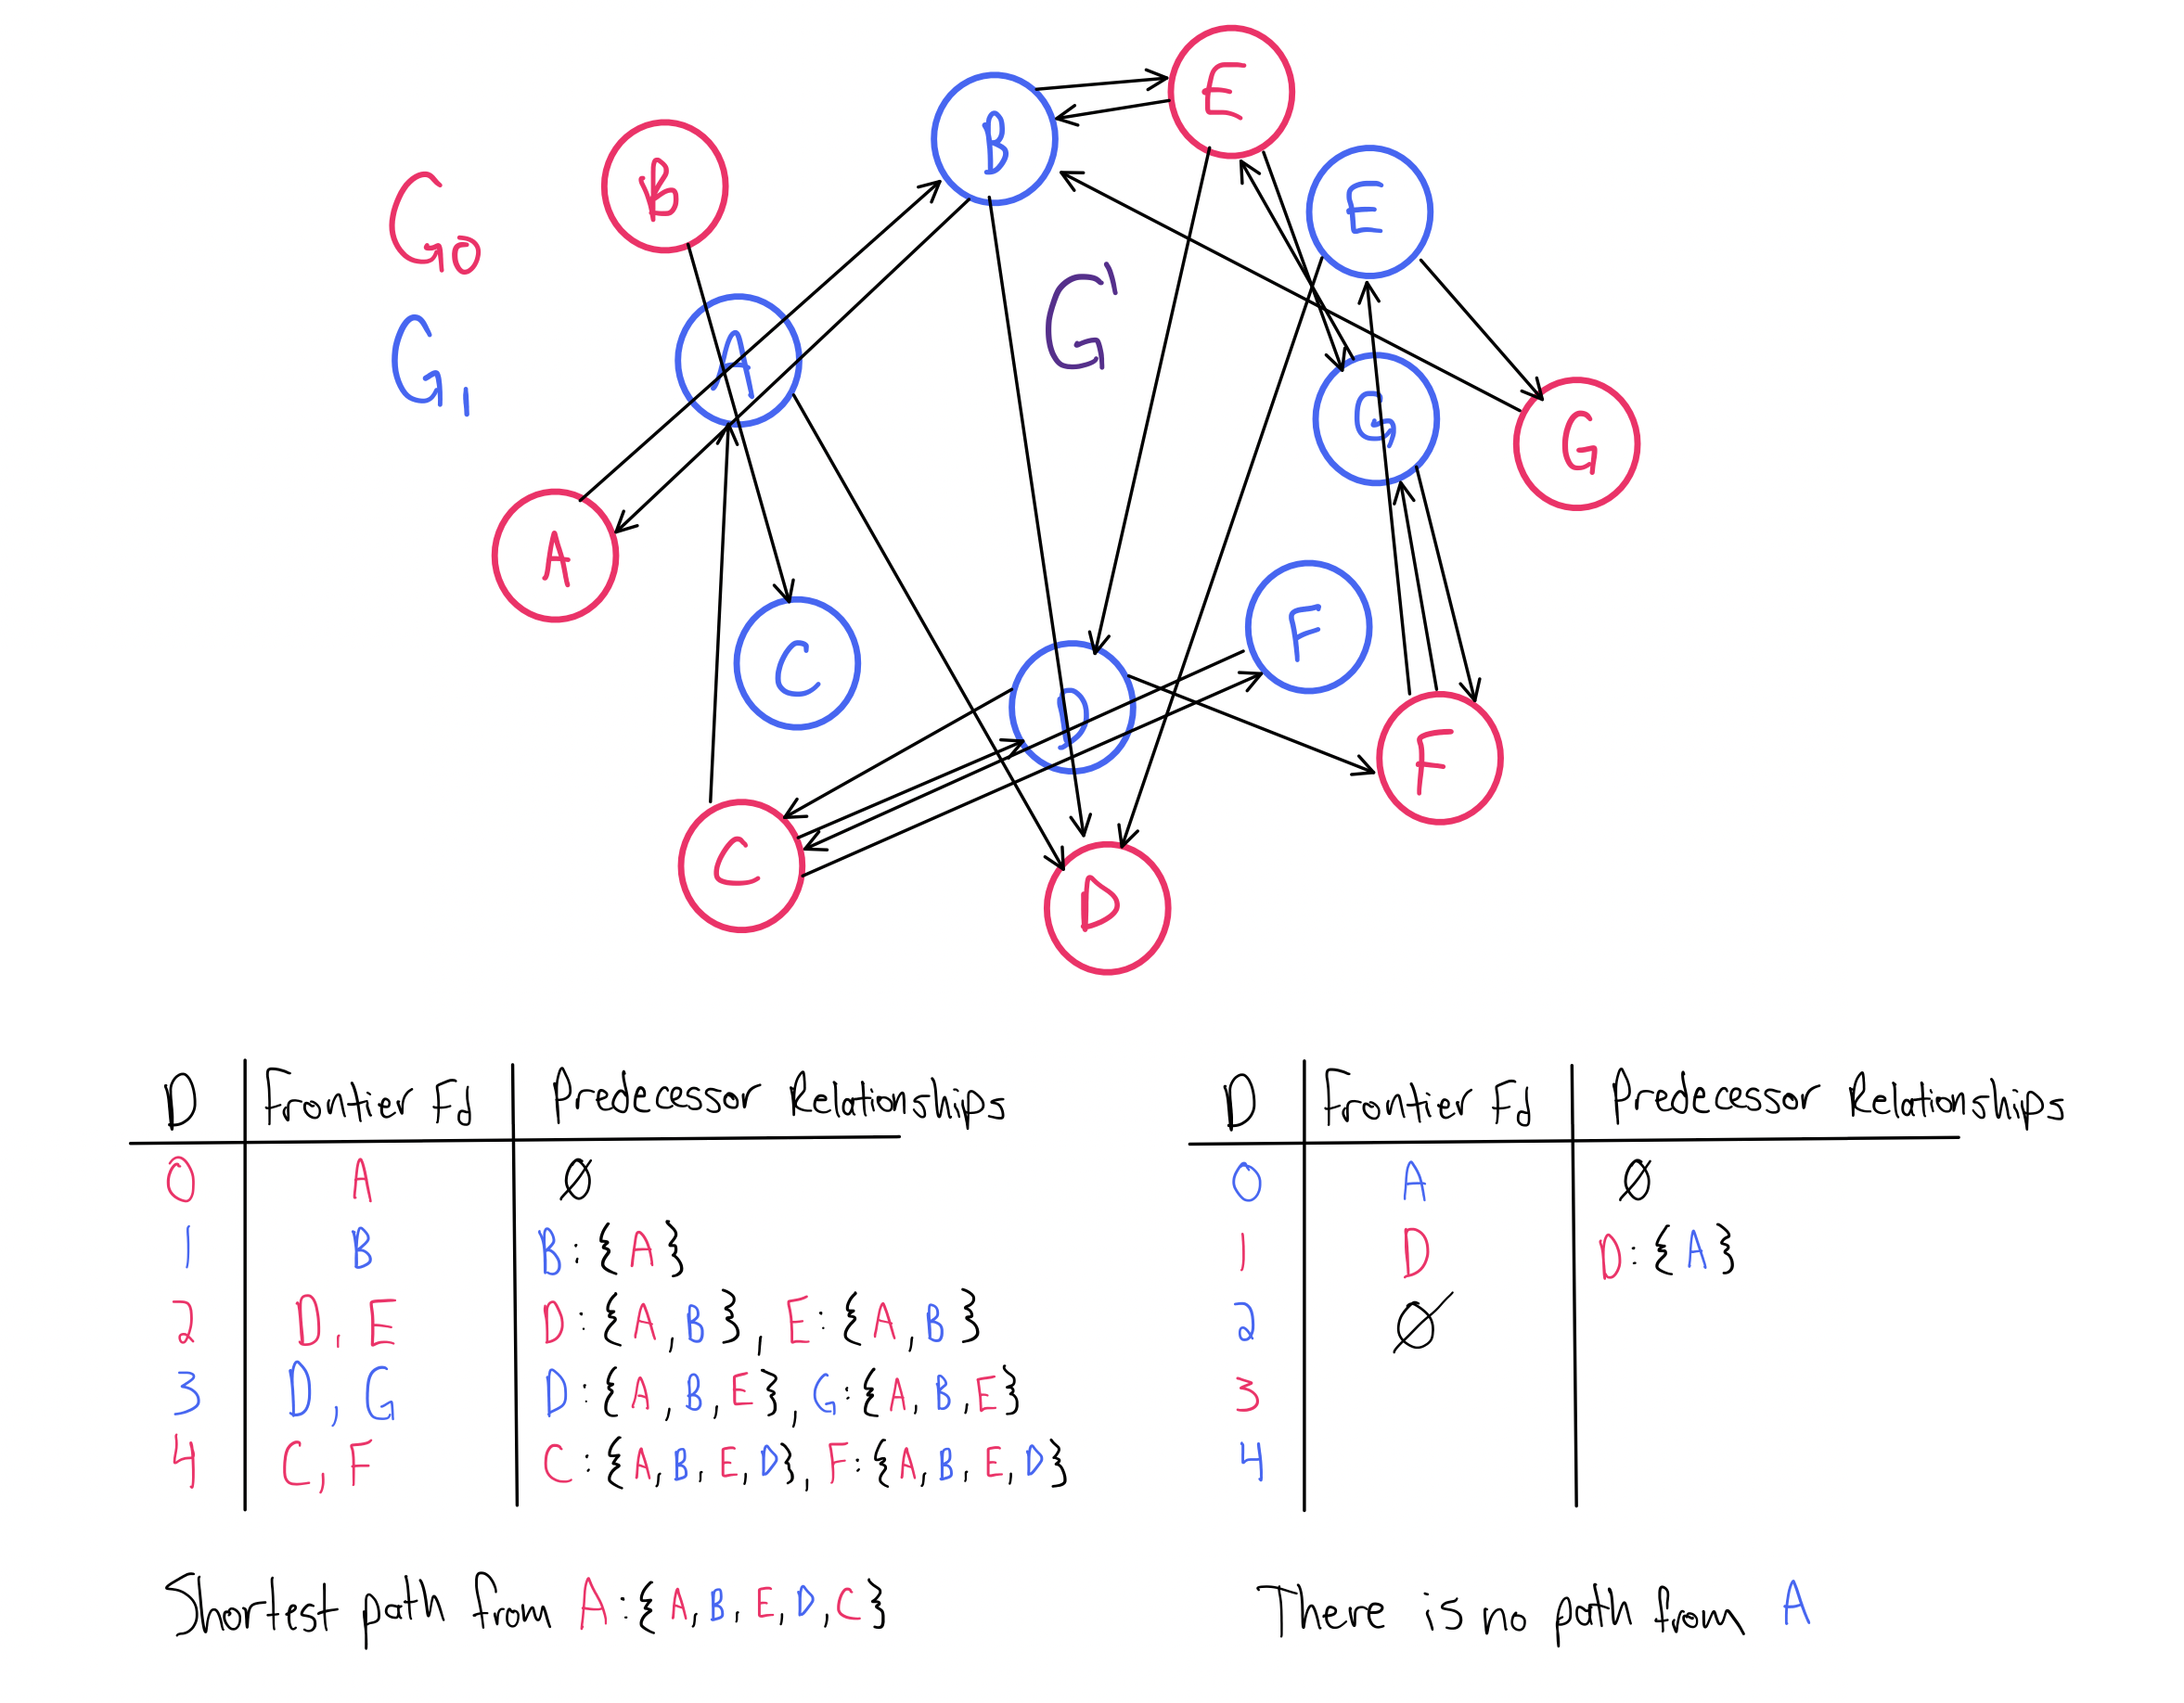
\includegraphics[scale=0.4]{3 b 2.png} 
       \newline
       \begin{quote}
           \color{purple}
            Note. I realized after I saved the picture that the algorithm is only supposed to consider paths beginning in Graph 0. With that in mind, the table on the right side is irrelevant.
       \end{quote}
    \item 
        A group of three friends decides to play a new cooperative game (similar to the real-life board game Magic Maze).  They rotate turns moving a shared single piece on an $n\times n$ grid.  The piece starts in the lower-left corner, and their goal is to get the piece to the upper-right corner in as few turns as possible.  Many of the spaces on the grid have visible bombs, so they cannot move their piece to those spaces.  Each player is restricted in how they can move the piece.  Player 0 can move it like a chess rook (any number of spaces vertically or horizontally, provided it does not cross any bomb spaces). Player 1 can move it like a chess bishop (any number of spaces diagonally in any direction, provided it does not cross any bomb spaces).  Player 2 can move it like a chess knight (move to any non-bomb space that is two steps away in a horizontal direction and one step away in a vertical direction or vice-versa).   Using Part~\ref{part:BFS}, show that given the $n\times n$ game board (i.e., the locations of all the bomb spaces), they can find the quickest solution in time $O(n^3)$.  
        (Hint: give a reduction, mapping the given grid to an appropriate instance $(G_0,G_1,\ldots,G_{k-1},s,t)$ of Shortest Rotating Walks.)
        \begin{quote}
            \color{purple}
            Consider the following algorithm, which assumes the $n$ by $n$ grid is a zero indexed coordinate plane with $(0, 0)$ at the bottom left and $(n - 1, n - 1)$ at the top right: 
            \vspace{1em}
            \begin{itemize}
                \item If $n < 1$, return $\bot$. If $n = 1$, return $[]$.
                \item Initialize three directed graphs: $G_{Rook}$, $G_{Bishop}$, and $G_{Knight}$. 
                \item For each index $i, j$ in the $n$ by $n$ grid:
                \begin{itemize}
                    \item For each $piece$ of $Rook$, $Bishop$, $Knight$:
                    \begin{itemize}
                        \item Add the $(i, j)$ index as a vertex to $G_{piece}$.
                        \item Add to $G_{piece}$ every edge beginning at $(i, j)$ and ending at a position $(x, y) \in n - 1 \times n - 1$ such that $(x, y)$ does not contain a bomb, can be reached by the piece in one move, and can be reached without crossing a bomb.
                    \end{itemize}
                \end{itemize}
                \item Call $ShortestRotatingWalks$ with $G_{Rook}$, $G_{Bishop}$, and $G_{Knight}$ such that the rotating walk should begin at $(0, 0)$, the bottom left, and end at $(n - 1, n - 1)$. Return this shortest walk. 
            \end{itemize}
            \vspace{1em}
            The algorithm relies heavily on abstraction, but details can be expanded. For example, temporary pointers can iterate diagonal indices from the Bishop's location in four different directions to determine reachable states, stopping early if a bomb is in the way. Similar ideas can be expanded for all three pieces. \newline 
            
            For this algorithm, the bomb grid is the only input. So, for any valid input grid of size $n$, the algorithm constructs three graphs containing every possible move each of the three pieces can make from every possible position. The call to $ShortestRotatingWalks$ begins with Player 0's Rook piece, and the shortest rotating walk from that position to the top right is returned (if one exists). Because the input graphs exhaustively consider the nodes and edges in the graph and $ShortestRotatingWalks$ is correct, this algorithm must return a valid output for every valid input, making it correct. \newline 

            \textbf{Runtime}: \newline 
            Runtime can be examined by breaking apart the stages of this algorithm: 
            \begin{itemize}
                \item Initial Preprocessing: The $n$ by $n$ grid is iterated for all three pieces. For both the Rook and Bishop, up to $2n$ edges may be added at each step. So, the preprocessing loop takes $O(n \cdot n \cdot 2n) = O(n^3)$ time to complete.
                \item $ShortestRotatingWalks$: This algorithm takes time $O(kn' + m_0 + m_1 + \dots + m_{k - 1})$ with a single reduction to $SingleSourceShortestWalk$. In this context, we know $k$ is $3$ because there are three input graphs. Each input graph contains $n^2$ vertices, so $kn = 3n^2$. Because every tile of every piece could potentially have an edge with every other tile on the board, each piece could have up to $n^3$ edges in its graph. With three pieces, the total reduction complexity in this case is $O(3n^2 + 3n^3) = O(n^3)$.
                \item From lecture, assert that $SingleSourceShortestWalk$ can be solved in time $O(n' + m)$, where $n'$ is the number of vertices and $m$ is the number of edges. In this case, the number of vertices is at most $3n^2$, and the number of edges is at most $3n^3$. That gives $SingleSourceShortestWalk$ complexity of $O(n^2 + 3n^3) = O(n^3)$.
            \end{itemize}
            \vspace{1em}
            Considering these together, initial preprocessing takes time $O(n^3)$. This is added to the runtime of $ShortestRotatingWalks$. Preprocessing for $ShortestRotatingWalks$ takes time $O(n^3)$ before $SingleSourceShortestWalk$ is called, which takes $O(n^3)$ time. Each of these functions is called once for any size $n$, so the overall complexity is $O(n^3 + n^3 + n^3)$, which simplifies to $O(n^3)$. Thus, the time complexity of this algorithm is $O(n^3)$.
            
        \end{quote}

 \end{enumerate}
 
\end{enumerate}
\end{document}
